\documentclass[12pt,a4paper,oneside]{book}
    \usepackage[utf8]{inputenc}
    \usepackage[english]{babel}
    \usepackage{amsmath}
    \usepackage{amssymb}
    \usepackage{amsthm}
    \usepackage{graphicx}
    \usepackage{hyperref}
    \usepackage[top=1in, bottom=1.25in, left=1.25in, right=1in]{geometry}
    \usepackage{wrapfig}
    \theoremstyle{definition}
    \newtheorem{definition}{Definition}[section]
    % \theoremstyle{remark}
    % \newtheorem*{remark}{Remark}
    % \newtheorem*{theorem}{Theorem}
    \usepackage[autostyle]{csquotes}
    \usepackage{float}
    \usepackage[font={small,it}]{caption}
    \usepackage[title]{appendix}
    \usepackage{subfig}
    \usepackage[export]{adjustbox}
    \usepackage{tikz}
    \usepackage{setspace}
    %\setlength{\parindent}{10pt}
    %\setlength{\parskip}{10pt}
    \usepackage{xcolor}
    \hypersetup{
        colorlinks,
        linkcolor={black!40!black},
        citecolor={blue!100!black},
        urlcolor={blue!80!black}
    }
    \renewcommand{\arraystretch}{2.5}
    \title{
        \sc
    \Huge{Skeleton Expansion }\\
    \Large{IN}\\%%in $d=6-\epsilon$%%}
    \Huge{Conformal Field Theory}
    % \\[5pt]
    % \Large{FOR}
    % \\[5pt]
    % \Huge{$\phi^3$ theory}
	\\[40pt]
	\large{A Thesis submitted for the completion of}
	\\[5pt]
	\large{requirements for the degree of}
	\\[15pt]
	\Large{Bachelor of Science}
	\\[5pt]
	\Large{(Research)}
	\\[40pt]
	\normalsize{by}
	\\[15pt]
	\large{Biplab Mahato}
	\\[5pt]
	\normalsize{Undergraduate Programme}
	\\[5pt]
	\normalsize{Indian Institute of Science}
	\\[40pt]
	\includegraphics[scale=0.15]{image/iisclogo.jpg}
	\\[40pt]
	\normalsize{Under the supervision of}
	\\[10pt]
	\large{Prof. Aninda Sinha}\\
    \normalsize{Indian Institute of Science}\\[5pt]
    \large{Prof. Biplob Bhattacharjee}\\
    \normalsize{Indian Institute of Science}
    \newpage
    }
    \author{}
    \date{}
    \begin{document}
        \singlespacing
        \begin{titlepage}
        \maketitle\clearpage
        \end{titlepage}
        \onehalfspacing
        \frontmatter
        \setlength{\parskip}{5pt}
        \chapter*{\centering Acknowledgement}
        \addcontentsline{toc}{chapter}{Acknowledgement}
            \hspace{15pt} I would like to thank the Undergraduate program at Indian Institute of Science for providing an excellent environment which deepened my curiosity in science and research in general.\par
            My whole hearted gratitude to my supervisor prof. Aninda Sinha for his guidance, encouragement and insightful discussions which made this thesis a reality. My warm gratitude to prof. Biplob Bhattacharjee for supervising the project. A big thank you to prof. Vasco Goncalves for clarifying doubts regarding his paper and sharing some of his Mathematica notebooks. Also my thanks to Kaushik Ghosh for meaningful discussions towards the begining of this project.\par
            I would also like to thank my faculty advisor prof Banibrata Mukhopadhyay for encouraging and motivating me in research in every single meeting that we had.  \par
            Finally I would like to thank my family and friends for supporting throughout my stay at IISc and making this four-year journey worth remembering.
        \chapter*{\centering Abstract}
        \addcontentsline{toc}{chapter}{Abstract}
            Conformal Field Theory, a quantum field theory exhibiting conformal symmetry, provides tight constraints on the correlation function at the critical point. These constraints are used to study and simplify skeleton expansion of $\phi^3$ theory in $6-\epsilon$ dimension. Using skeleton diagrams we have computed the four-point function up to $O(\epsilon^2)$. This allows us to calculate CFT data for the theory, using conformal block decomposition. CFT data can also be recovered from the large spin bootstrap method or equivalently from inversion integral derived by Caron-Huot. These methods are also studied and the final result is matched with the previously calculated OPE data and anomalous dimensions.
        
        \tableofcontents
        \mainmatter
        \chapter{Introduction}
            \hspace{10pt}The idea of critical points, where the distinction between liquid and gas gets blurred, was introduced by Thomas Andrews~\cite{critical}. Since then many systems exhibiting critical pheonemenon are studied extensively. In 1908 Marian Smoluchowski~\cite{longdistance} noticed that density fluctuations correlate to longer and longer distances as one approaches the critical point. This introduced the idea of power law behaviour of correlation function near critical points rather than an exponential drop-off. Interestingly enough, these exponents turned out to be the same for a remarkable number of seemingly unrelated systems. This leads to the concept of Universality classes. Origin of universality is usually explained by the renormalisation group methods~\cite{RG}. This method can also be used to calculate the critical exponents. Traditionally, the method requires evaluation of Feynman diagrams, renormalisation of operators and computation of the so called $\beta$ function. $\epsilon$-expansion~\cite{epsilonexpansion} enable this method to be applicable to almost all the systems. Although the method is really tedious and it is almost impossible to extend an existing theory beyond a few orders in $\epsilon$.  \par
            In 1970 Polyakov~\cite{polyakovsymmetry} building on the work of Mack and Salam~\cite{mack-salam} conjectured that at critical point systems acquire an enhanced cornformal symmetry. Based on this conformal symmetry one can heavily simplify the computaions in RG methods by using an improved Feynman Diagram method known as Skeleton Diagrams. This method allows a simple straight-forward evaluation of correlation functions. \par 
            Along with that, conformal symmetry gave rise  to a new branch of field theory known as  the Conformal Field Theory. Conformal field theory is charecterised by a collection of local primary operators satisfying an algebra called the operator product expansion. Structure constant of the algebra along with the labels of the  operators(scaling dimension and spin) constitute the CFT data. CFT data  encodes all the information about the critical exponents. Hence it is enough to focus on calculating CFT data. \par
            % Bootstrap methods are known for a very long time. Since the introduction of a few consistency relations by Polyakov~\cite{polyakov} many have improved the techniques to obtain CFT data. Unitarity, Crossing symmetry, analyticity provide many results and constraints to the thoery. Analyticity in spin introduces an inversion formula~\cite{inversiongravitation} to obtain OPEs solely from the discontinuties of the correlators.  \par
            Bootstrap idea was first advocated by Geoffrey Chew in 1950s. His belief was that the theory of nature is the only theory consistent with it, that is to say that, consistency relation alone is enough to build up the theory of everything. Using this bottom-up approach he was able to successfully predict the mass of rho meson. Although in other cases this method failed miserably. In 1970 Polyakov\cite{polyakov}, Ferrara, Gatto introduced conformal symmetry into the theory and was able to derive few more consistency relations. This laid the foundation of Conformal Bootstap, a bottom-up, non-perturbative theory, derived solely from first principles. But the theory beyond two dimensions, seemed so complicated that progress in the field merely stopped. In 2008 Rychkov, Rattazzi, Tonni and Vichi\cite{rychkov} revived the theory with a new approach. Instead of looking for the unique answer to conformal bootstrap equations they devised a way to rule out plausible theories based on consistency conditions. Many numerical techniques since then applied to map the region of allowed theories. Analytical tools have also become more powerful. Unitarity, Crossing Symmetry of four point function introduced more consistency relations. Crossing symmetry is typically explored in two main methods. One uses exchange Witten diagram in Mellin space\cite{aninda} to decompose four point function. While the other uses analyticity in spin  to solve bootstrap equations as a perturbation from large spin operator. The latter is extended to obtain an inversion formula\cite{inversiongravitation} to calculate CFT data from the singularities of the correlators.\par
            The aim of this thesis is to obtain CFT data for $\phi^3$ theory in $(6-\epsilon)$ dimension using the method of skeleton diagrams following a paper by Vasco Goncalves \cite{vasco}. We have also obtained the anomalous dimensions and OPE coefficients using the inversion formula and matched two of the results. \par
            The text is mainly divided into four parts. In chapter \ref{basics} basic ideas of Conformal Field Theory($d\geq3$) is briefly stated. This part lay the foundations to understand the rest of the text. Although certain familiarity of Quantum Field Theory and Lie algebra is assumed. Next in chapter \ref{skeleton} we used skeleton expansion to obtain the four point function upto order $\epsilon^2$. The result from this is used in chapter \ref{conformal-block-decomposition} to obtain the OPE co-efficients as well as the anomalous dimensions of the operators appearing in the theory. In chapter \ref{inversion-integral} Bootstrap technique is introduced along with the inversion formula. Using inversion formula we again calculate the anomalous dimensions and OPE co-efficients.
        \chapter{Basics of CFT}\label{basics}
        \section{Conformal Symmetry}
        Conformal Field Theory can be defined to be the Quantum Field Theory which is invariant under conformal transformations. Conformal transformations are those maps which locally preserve orientation and angles. That is to say, a map $f: U\to V$ is called conformal if for any point $u\in U$, directed curves passing through it, have the same angle between them when mapped to $V$ via $f$. It is convenient to think $U$ and $V$ to be subspaces of same ambient space. These transformations, in general, do not keep the metric invariant but rather introduce multiplicative factor depending on the coordinate of the point.
        \begin{equation}
            x\to f(x) = x';\hspace{5pt} g_{\rho\sigma}'(x')\frac{\partial x'^{\rho}}{\partial x^{\mu}}\frac{\partial x'^{\sigma}}{\partial x^{\nu}} = \omega^2(x)g_{\mu\nu}(x)
        \end{equation}
        In a locally Minkowskian reference frame the last relation take the form $\eta_{\rho\sigma}\frac{\partial x'^{\rho}}{\partial x^{\mu}}\frac{\partial x'^{\sigma}}{\partial x^{\nu}} = \omega^2(x)\eta_{\mu\nu}$. Transformations allowed by this equation are categorised into following four types.
        \begin{itemize}
            \item \textbf{Translation} $x'^{\mu} = x^{\mu} + a^{\mu}$ 
            \item \textbf{Rotation} $x'^{\mu} = M_{\nu}^{\mu} x^{\nu}$ where $M_{\nu}^{\mu}$ is rotation matrix which also includes space-time rotations.
        \end{itemize}
            Apart from the above transformations, which are also present in the Poincare group,  there are two more additional transformations.
        \begin{itemize}
            \item \textbf{Dilation} $x'^{\mu} = \alpha x^{\mu}$ where $\alpha>0$.
            \item \textbf{Special Conformal Transformation(SCT)} $x'^{\mu} = \frac{x^{\mu}-(x\cdot x)b^{\mu}}{1-2(b\cdot x)+(b\cdot b)(x\cdot x)}$\footnote{This can also be wrtiien as $\frac{x'^{\mu}}{(x'\cdot x')} = \frac{x^{\mu}}{(x\cdot x)}-b^{\mu}$ which can then be interpreted as an inversion of $x^{\mu}$ followed by translation $b^{\mu}$ and then inversion back}
        \end{itemize}
        It is easy to check that these form a group under the composition map as multiplication. Also all these transformations are labeled by various parameters. Note that the transformations are smooth (differentiable infinite times) with respect to each parameters and identity transformation arises when parameters goes to zero (for dilation we can reparameterise $\alpha$ as $e^{t}$). These make the set of all those transformations a Lie group (Conformal Group).
    % To understand how these transformation affect the fields we make the following definations (they can be justified by requiring a representation of the Lie algebra associated with the Conformal group)
    % \begin{definition}[Scaling Dimension]
    %     If under the dialation $x\rightarrow x'=\lambda x$ a field transform as $\phi(x)\rightarrow \phi'(x') = \lambda^{-\Delta}\phi(x)$ then $\Delta$ is called the \emph{scaling dimension} of the theory.
    % \end{definition}
    % In fact one can make even a stronger definition
    % \begin{definition}[Quasi-Primary Field]
    %     A \emph{quasi-primary field} is a field in dimension $d$ which transform under the co-ordinate transformation $x\rightarrow x'$ as 
    %     \begin{equation}
    %         \phi(x)\rightarrow\phi'(x') = \bigg\lvert \frac{\partial x'}{\partial x} \bigg\rvert^{-\Delta/d} \phi(x)
    %     \end{equation}
    % \end{definition}
    % Consider the case of special conformal transformation. Jacobian for this case becomes
    % \begin{equation}
    %     \bigg\lvert \frac{\partial x'}{\partial x} \bigg\rvert = \frac{1}{(1-2(b\cdot x)+(b\cdot b)(x\cdot x))^{d}}
    % \end{equation} 
    % and distances transform as
    % \begin{equation}
    %     \lvert x_{i} - x_{j} \rvert \rightarrow \frac{\lvert x_{i} - x_{j} \rvert}{(1-2(b\cdot x_{i})+(b\cdot b)(x_{i}\cdot x_{i}))^{1/2}(1-2(b\cdot x_{j})+(b\cdot b)(x_{j}\cdot x_{j}))^{1/2}}
    % \end{equation}
    \section{Conformal Algebra}\label{conformal algebra}
    It is always enlightening to look at the Algebra associated with a Lie group. To do so first consider the infinitesimal version of each transformations. From them one can easily identify the generators of the group. We will label generators of translations as $P_{\mu}$, of rotations as $M_{\mu\nu}$, of dilation as $D$ and of SCT's as $K_{\mu}$. These generators have following form
    % Before procedding further we must have more understanding of the Hilbert space where we are operating. Hilbert space as known, is the space\footnote{mathematically any space having an inner product and being complete with respect to the distance function derivable from the scalar product is a Hilbert space but physics (Unitarity, Causality etc.) only allows very special kind of spaces (e.g. only Separable (existence of countable basis) once are mostly relevent in physics)} containing all the states. To 'construct' the Hilbert space better understanding of the symmetries is necessary. Conformal symmetries form a Lie group (groups having geometrical structures). It is always enlightening to look at the Lie algebra associated with it.\\
    % In Conformal Algebra we have the usual translation genetator $P_{\mu}$ and the Lorentz boost generators (with the rotations) $M_{\mu \nu}$. Along with them we have the generators for dilation $D$ and for special conformal transformation written as $K_{\mu}$. Their form is given below
    \begin{subequations}
    \begin{align}
        P_{\mu} &= -i \partial_{\mu}\\
        M_{\mu\nu} &= i \left(x_{\mu}\partial_{\nu} - x_{\nu}\partial_{\mu} \right)\\
        D &= -i x^{\mu}\partial_{\mu} \\
        K_{\mu} &= -i \left(2x_{\mu}(x^{\nu}\partial_{\nu}) - x^2\partial_{\mu} \right)
    \end{align}
    \end{subequations}
    From the form of the generators one can then easily compute the commutators which will constitute the Lie Algebra(Conformal Algebra).
    \begin{subequations}
    \begin{align}\label{liealgebra}
        \left[M_{\mu\nu},M_{\rho\sigma} \right] &= i\left(\eta_{\nu\rho}M_{\mu\sigma} \pm permutations  \right)\\
        \left[M_{\mu\nu},P_{\rho} \right] &= i \left(\eta_{\rho\nu}P_{\mu} - \eta_{\rho\mu}P_{\mu} \right)\\
        \left[M_{\mu\nu},K_{\rho} \right] &= i \left(\eta_{\rho\nu}K_{\mu} - \eta_{\rho\mu}K_{\mu} \right)\\
        \left[K_{\mu},P_{\nu} \right] &= 2i \left(\eta_{\mu\nu}D - M_{\mu\nu} \right)\\
        \left[D,P_{\mu} \right] &= i P_{\mu}\\
        \left[D,K_{\mu}\right] &= -i K_{\mu}
    \end{align}
\end{subequations}
    These relations can be identified with the algebra of $SO(d+1,1)$\cite{lecturenote}\cite{textbook}.  
    The first two commutation relation is the same as Poincare algebra. The last two will be used later in the text.
    \section{Algebra action on operators}
    Now consider a scalar field $\phi(x)$ defined on the space-time. After quantisation, this field will become an operator. Under a scale transformation, this field transform as 
    \begin{equation}
        x\to x'=\lambda x;\hspace{10pt} \phi(x)\to \lambda^{-\Delta}\phi(x)
    \end{equation}
    where $\Delta $ is called the scaling dimension of the field. This can be generalised for any transformation by replacing the factor with the Jacobian.
    \begin{equation}
        \phi(x)\rightarrow\phi'(x') = \bigg\lvert \frac{\partial x'}{\partial x} \bigg\rvert^{-\Delta/d} \phi(x)
    \end{equation}
    % Now we are  ready to derive the action of the generators on the operators. Recall that we have for scalars
    % \begin{equation}
    %     x \to x' , \hspace{10pt} \phi(x)\to \phi(x') = \frac{1}{b(x)^{\Delta}}\phi(x)
    % \end{equation}
    Now consider an infinitesimal transformation $x'^{\mu} = x^{\mu} + \epsilon^{\mu}$. This gives $\phi'(x') = (1+\partial_{\mu}\epsilon^{\mu})^{-\Delta}\phi(x)$.\par
    Expanding fields upto first order for a specific generator $G$ (corrospondingly $\epsilon^{\mu}$)
    \begin{equation}
        (1+\partial_{\mu}\epsilon^{\mu})^{\Delta} \phi(x') = \phi(x) + \epsilon(G\phi(x))
    \end{equation}
    where $G\phi$ represents the action of $G$ on $\phi$. The above expression yeilds
    \begin{equation}
        G\phi(x) = (\Delta\partial_{\mu}\epsilon^{\mu})\phi(x) + \epsilon^{\mu}\partial_{\mu}\phi(x)
    \end{equation}
    We know $\epsilon^{\mu}$ for each generators, using that now we can derive the algebra action on the fields. Also in QFT action of a generator $G\phi$ is written as a commutator $[G,\phi]$. So we get the following actions of generators on the operator $\mathcal{O}$
    \begin{subequations}
    \begin{align}\label{algebra-action}
        \left[P_{\mu},\mathcal{O}(x) \right] &= -i \partial_{\mu} \mathcal{O}(x)\\
        \left[D,\mathcal{O}(x) \right] &= -i\left(\Delta + x^{\mu}\partial_{\mu} \right)\mathcal{O}(x)\\
        \left[M_{\mu\nu},\mathcal{O}(x) \right] &= -i \left(\Sigma_{\mu\nu} +x_{\mu}\partial_{\nu} - x_{\nu}\partial_{\mu} \right)\mathcal{O}(x)\\
        \left[K_{\mu},\mathcal{O} \right] &= -i\left(2x_{\mu}\Delta + 2x^{\lambda}\Sigma_{\lambda\mu} + 2x_{\mu}(x^{\rho}\partial_{\rho} - x^2\partial_{\mu}) \right)\mathcal{O}(x)
     \end{align}
    \end{subequations}
    \section{Radial Quantisation}
    One of the main ideas of QFT is  `foliation' of space-time. That is to consider $d-1$ dimensional subspaces of $d$ dimensional subspace, each subspace endowed with their own Hilbert space structure. The chosen one  dimensional subspace  used to foliate space-time plays a special role in the theory. For example, in traditional QFT, it is the time that serves the purpose of foliation. We have then $(d-1)$ dimensional time slices. One can travel through different slices using the Hamiltonian operator ($U = e^{iHt}$). Similar foliation is also required in CFT. Note that time can be chosen to foliate space-time in CFT, but it has further symmetries and choosing dialation operator for foliation is much more convinient(traditional). This foliates the space-time into $d-1$ dimensional spheres($S_{d-1}$) around the origin (arbitrary just like the zero in the time axis). States on the sphere are classified by their scaling dimension and spin (coming from $SO(d-1)$ representation).
    \begin{subequations}
    \begin{align}
        D|\Delta\rangle &= i\Delta|\Delta\rangle\\
        M_{\mu\nu} |\Delta,l\rangle &= \left(\Sigma_{\mu\nu}\right)|\Delta\rangle
    \end{align}
\end{subequations}
    \section{State-operator correspondence}
    Now we are ready to construct states in the space. First and foremost the vacuum state $|0\rangle$\footnote{this is consistent with the earlier notation as vacuum state is the eigenstate of dilatation operator with 0 as eigenvalue} which corresponds to no operator insertions at the origin. Also, it is assumed that the vacuum state is unique and is invariant under all global conformal transformations. So using the operator action on the field \ref{algebra-action} we conclude that the operator $\mathcal{O}_{\Delta}(x=0)$ when inserted at the origin it produces a state $|\Delta\rangle$. Similarly, for each operator, we can produce a state corresponding to it. 
    \par
    In converse given a state, we can also construct an operator. To do so note that defining an operator is equivalent to define all its n-point functions. That can be done as below
    \begin{equation}
        \langle\phi (x_{1}) \phi(x_{2})\cdots\mathcal{O}_{\Delta}(0)\rangle := \langle 0|\phi(x_1)\phi(x_2)\cdots |\Delta\rangle
    \end{equation}
    This one-one mapping is known as the \emph{state-operator correspondance}.
    \subsection*{Primary and descendants}
        From the algebra of generators one can easily see that $P_{\mu}$ and $K_{\mu}$ acts on the state as raising and lowering operators respectively.
        \begin{align}
            DP_{\mu}|\Delta\rangle &= P_{\mu}D|\Delta\rangle + [D,P_{\mu}]|\Delta\rangle = i(\Delta+1)P_{\mu}|\Delta\rangle\nonumber\\
            DK_{\mu}|\Delta\rangle &= K_{\mu}D|\Delta\rangle + [D,K_{\mu}]|\Delta\rangle = i(\Delta-1)K_{\mu}|\Delta\rangle
        \end{align}
        So each time $K_{\mu}$ is acted upon a state its scaling dimension decreases by one. By unitarity (see \ref{unitary})scaling dimension cannot be negative. So eventually $K_{\mu}$ must annihilate the state. The state which gets annihilate by the action of $K_{\mu}$ is called primary state (corrospondingly primary operator) and all the states obtained from it by acting $P_{\mu}$ repeatedly are called descendants. Primary operaotors and all of its descendants consitute the so called \emph{conformal family}. Also note that scaling dimensions can only be positive integers\footnote{scaling dimension will get corrections (anomalous dimensions) in an interacting theory}.
    \subsection*{Unitary Bounds}\label{unitary}
        States are charecterised by their scaling dimensions. Unitarity of the theory poses tight constraints on those scaling dimensions. To derive those constraints we first need the fact that $P_{\mu}^{\dagger} = K_{\mu}$. \par
        Consider a state with scaling dimension $\Delta$ corresponding to a scalar field ($M_{\mu\nu}|\Delta\rangle = 0$)
        \begin{align}
            \langle\Delta|K_{\mu}P_{\nu}|\Delta \rangle &= \langle\Delta|[K_{\mu},P_{\nu}]|\Delta\rangle  + \langle\Delta|P_{\nu}K_{\mu}|\Delta\rangle\nonumber\\
            &= 2i\langle\Delta|D\eta_{\mu\nu}-M_{\mu\nu}|\Delta\rangle\\
            &= \Delta\eta_{\mu\nu}\nonumber
        \end{align}
        As K and P are Hermitian conjugate of each other $\langle\Delta|K_{\mu}P_{\nu}|\Delta \rangle$ is just the norm of the state $P_{\nu}|\Delta \rangle$. By unitarity this has to be non-negative which implies $\Delta\geq 0$.\par
        Further tight constraints can be derived considering similar inner product of states. Tightest of these are 
        \begin{subequations}
        \begin{align}
            \Delta -l &\geq d-2\hspace{20pt}l\neq 0\\
            \Delta &\geq \frac{d-2}{2}\hspace{20pt}l=0
        \end{align}
    \end{subequations}
    \section{Correlation functions}
    Using results from the previous section and requiring conformal invariance we can now derive the correlation functions 
    \subsection{Two-point function(Propagator)}\label{propagator}
        Two point correlation function $\langle\phi_{i}(x_1)\phi_{j}(x_2)\rangle$ should in principle depend on the position $x_1$ and $x_2$. But translation invariance implies that the dependence should be on their difference. Other Poincare invariance implies that it should depend on the $\lvert x_1 - x_2 \rvert$ (for brevity $x_{12}$). Now on co-ordinate transformation two-point function should transform as
        \begin{equation}
            \langle\phi'_{i}(x'_1)\phi'_{j}(x'_2)\rangle = \bigg\lvert \frac{\partial x'}{\partial x} \bigg\rvert_{x=x_1}^{-\Delta_{1}/d} \bigg\lvert \frac{\partial x'}{\partial x} \bigg\rvert_{x=x_2}^{-\Delta_{2}/d} \langle\phi_{i}(x_1)\phi_{j}(x_2)\rangle 
        \end{equation}
        Also we have $\langle\phi_{i}(x_1)\phi_{j}(x_2)\rangle = f(x_{12})$. Under the dialation (scaling) transformation $x\rightarrow \lambda x$ if $f$ has to remain invariant then we need
        \begin{equation}
            f(x) = \lambda^{\Delta_1 + \Delta_2} f(\lambda x)
        \end{equation} 
        This forces f to be of the form 
        \begin{equation}
            f(x_{12}) = \frac{d_{ij}}{(x_{12})^{\Delta_1 + \Delta_2}}
        \end{equation}
        Now requiring conformal invariance we have
        \begin{equation}
            \frac{d_{ij}}{(x_{12})^{\Delta_1 + \Delta_2}} = \frac{d_{ij}(\gamma_1\gamma_2)^{(\Delta_1+\Delta_2)/2}}{\gamma_1^{\Delta_1}\gamma_2^{\Delta_2}x_{12}^{\Delta_1 + \Delta_2}}
        \end{equation}
        where $\gamma_i = (1-2(b\cdot x_i)+(b\cdot b)(x_i \cdot x_i))$. From the above equation it is clear that we must have $\Delta_1 = \Delta_2$. Also then we can rescale the field itself to make $d_{ij} = \delta_{ij}$. Finally we obtain 
        \begin{equation}
            \langle\phi_{i}(x_1)\phi_{j}(x_2)\rangle = \frac{\delta_{ij}}{(x_{12})^{2\Delta_1}}
        \end{equation}
    \subsection{Three-point function}\label{3ptfunction}
        For the case of three point function we can proceed similarly. We should have that $\langle\phi_{i}(x_1)\phi_{j}(x_2)\phi_{k}(x_3)\rangle = f_{ijk}(x_{12},x_{23},x_{13})$ for some function $f$. By requiring scale invariance we obtain the form
        \begin{equation}
            f_{ijk}(x_{12},x_{23},x_{13}) = \frac{C_{ijk}}{x_{12}^{a}x_{23}^{b}x_{13}^{c}}
        \end{equation}
        where we need $a+b+c = \Delta_1 + \Delta_2 + \Delta_3$. Special conformal invariance can then be used just like previous case to obtain 
        \begin{align*}
            a = \Delta_1 + \Delta_2 - \Delta_3\\
            b = \Delta_2+\Delta_3-\Delta_1\\
            c = \Delta_1+\Delta_3-\Delta_2
        \end{align*}
        Using concise notation $\Delta_{ij,k} := \Delta_i+\Delta_j-\Delta_k$ we have the three point correlation function
        \begin{equation}
            \langle\phi_{i}(x_1)\phi_{j}(x_2)\phi_{k}(x_3)\rangle = \frac{C_{ijk}}{x_{12}^{\Delta_{12,3}}x_{23}^{\Delta_{23,1}}x_{13}^{\Delta_{13,2}}}
        \end{equation}

\chapter{Skeleton Expansion}\label{skeleton}
    \section{Feynman Diagram for $\phi^3$ theory}
        Consider the Lagrangian density for massless scalar field with $\phi^3$ interaction.
        \begin{equation}
            \mathcal{L} = \frac{1}{2}\partial^{\mu}\phi\partial_{\mu}\phi - \lambda\phi^3
        \end{equation}
        From this we have the interacting part of the Hamiltonian to be $H_{I}(t) = \int d^dx(\lambda\phi^3) $\footnote{here we have assumed space-time to be d+1 dimentional for notational convenience}. In Perturbation Theory one then writes the following formula for n-point correlation function.
        \begin{equation}
            \langle\phi(x_1)\cdots\phi(x_n)\rangle = \lim_{T\to\infty(1+i\epsilon) } \frac{\langle0|\mathcal{T}\left\{\phi(x_1)\cdots\phi(x_n)exp\left[-i\int_{-T}^TdtH_I(t)\right] \right\}|0\rangle}{\langle0|\mathcal{T}\left\{exp\left[-i\int_{-T}^TdtH_I(t)\right] \right\}|0\rangle}
        \end{equation} 
    where $\mathcal{T}$ represent the time ordered product. Denominator of the equation removes all dis-connected diagrams. Connected diagrams comes from the terms like \begin{equation}\frac{\lambda^k}{k!}\langle0|\mathcal{T}\left\{\phi(x_1)\cdots\phi(x_n) (\phi(y_1)^3\cdots\phi(y_k)^3)\right\}|0\rangle.\end{equation} From this it is easy to see that for connected diagrams we must have each $x_i$'s connected to one of the $y_j$'s and remaining internal points are intertwined to make a connected graph. Also note that each vertex will have three lines connected to it. Feynman rules are also easy to write at this point but we skip it as we will not be using it.\par
        In principle, Feynman diagram for any order in $\lambda$ can be written which can be evaluated using Feynman rules. But with each order number of diagrams will keep on increasing and moreover many of the diagrams will have divergences which have to be renormalised by hand. This much hard-work can be heavily reduced using the concept of skeleton diagrams for the system exhibiting conformal symmetry\footnote{due to masslessness of the theory, it is scale-invariant and usually most scale-invariant theories are also conformal-invariant }  

    \section{Skeleton Diagram}
    Consider a planer Feynman diagram of order 4 or more. Any subgraph of this in $\phi^3$ theory will have 3 or less external lines. Now consider all possible subgraph with the given tree-level structure. It is easy to see that after summing all such diagrams one would just obtain complete irreducible 2 or 3 point function replacing the whole subgraph. That is one can just replace the vertices by respective complete 3-point vertex function (red blob just like~\ref{fig:vertex}). Algorithmically the procedure is(see \cite{srednicki} for details)
    \begin{enumerate}
        \item Sum all 1PI diagrams with two external lines. This will be used as propagator in the skeleton diagram.\label{one}
        \item Sum all 1PI diagrams with three external lines. In skeleton diagram the sum will replace the vertices.\label{two}
        \item For n-point function draw all 1PI diagrams with n external lines but omit diagrams which have propagators or vertex correction in the subgraph i.e. subgraphs are of less complexity than the tree-level diagrams.
        \item Use full propagator obtained in the (1) and V for any vertex from (2) to calculate the diagram.
    \end{enumerate}
    Note that this scheme although reduces the complexity of the diagram as well as potentially reduce the number of diagrams. But still, there is a mammoth task of performing (\ref{one}) and (\ref{two}). Without further symmetry or pattern in the individual terms sum, in general, cannot be calculated. Fortunately, conformal invariance allows us to calculate these immediately. \par
    First, consider the two-point function. Any propagator in CFT must have the form derived in \ref{propagator}. This tells us that the sum have to be equal to $\frac{1}{x_{12}^{2\Delta_{\phi}}}$. Although now $\Delta_{\phi}$ \footnote{throughout this chapter $\Delta_{\phi}$ is written as $\Delta$ to make the equation look less cumbersome}would not just be equal to 2, it will acquire some correction (re-normalised scaling dimension) known as anomalous dimensions.\par
    Similarly for 3 point functions, \ref{3ptfunction} tells us what the form of the sum will be. In section \ref{vertex} we will derive the explicit form of the vertex correction which will be used to evaluate skeleton diagram.\par
    This is a significant improvement as all the massive calculations that have to be done in (\ref{one}) and (\ref{two}) is already known. Also, this method does not give rise to any divergences as we are only dealing with physical quantities. So pain-staking renormalisation procedure is completely absent in this method.
    \section{Star-Triangle Formula}\label{startriangle}
    Before proceeding further we would like to introduce one of the most used Integrals in the text, the so-called \emph{Symanzik Star-Triangle Formula}\cite{symanzik}.
    \begin{equation}
        \boxed{
        \int \frac{d^{d}x_4}{x_{14}^{2\Delta_1}x_{24}^{2\Delta_2}x_{34}^{2\Delta_3}} = \frac{\kappa(\Delta_1,\Delta_2,\Delta_3)}{x_{12}^{\Delta_{12,3}}x_{23}^{\Delta_{23,1}}x_{13}^{\Delta_{13,2}}}}
    \end{equation}
    where $d = \sum_{i} \Delta_i$ and
    \begin{equation}
        \kappa(\Delta_1,\Delta_2,\Delta_3) = \pi^{\frac{d}{2}}\frac{\Gamma(\frac{\Delta_{12,3}}{2})\Gamma(\frac{\Delta_{23,1}}{2})\Gamma(\frac{\Delta_{13,2}}{2})}{\Gamma(\Delta_1)\Gamma(\Delta_2)\Gamma(\Delta_3)}
    \end{equation}
    \section{Vertex Correction}\label{vertex}

    To obtain vertex correction in the theory we consider the three-point function. This is because we know that in a $\phi^{3}$ theory all the vertex will have three propagators emanating from it. So consider a vertex as shown in the figure. We can assume that the correction to the vertex can be written as a function of three position variables. But we must have the following condition to be satisfied
    \begin{equation}
        \langle \phi_1(x_1)\phi_2(x_2)\phi_3(x_3) \rangle = \int \left(\prod_{i=1}^{3}dy_i\langle\phi_i(x_i)\phi_i(y_i)\rangle \right)V(y_1,y_2,y_3)
    \end{equation}
    \begin{wrapfigure}{r}{0.2\textwidth}
        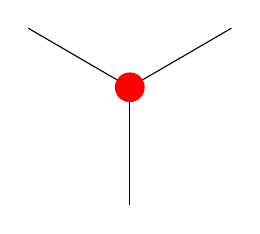
\begin{tikzpicture}[scale=1.5]
            \draw (0,0)--(0,1); 
            \draw (0,1)--(-0.86,1.5);
            \draw (0,1)--(0.86,1.5);
            \draw[red,fill=red] (0,1) circle (0.8ex);
        \end{tikzpicture}
        \caption{Three point function with dressed vertex}\label{fig:vertex}
    \end{wrapfigure}
    The vertex function can easily be determined by again requiring conformal invariance. Integrals are done using star-triangle formula. We obtain the vertex function to be
    \begin{equation}
        V(y_1,y_2,y_3) = \frac{g_{123}}{(y_{12}^2)^{\frac{d-\Delta_{12,3}}{2}}(y_{13}^2)^{\frac{d-\Delta_{13,2}}{2}}(y_{23}^2)^{\frac{d-\Delta_{23,1}}{2}}}
    \end{equation}
    where $d = \sum_{i=1}^3 \Delta_i$.\par
    When integral is done we also obtain a relation between $g_{123}$ and $C_{123}$.
    \footnotesize
    \begin{equation}
        C_{123} = g_{123}\kappa\left(\Delta_1,\tfrac{d-\Delta_{12,3}}{2},\tfrac{d-\Delta_{13,2}}{2} \right)\kappa\left(\tfrac{d-\Delta_{23,1}}{2},\tfrac{d-\Delta_{13,2}}{2},\Delta_3 \right)\kappa\left(\tfrac{\Delta_{13,2}}{2},\Delta_2,\tfrac{2d-\Delta_1-\Delta_2-\Delta_3}{2} \right)
    \end{equation}
    \normalsize
    \section{Tree-Level calculaitons}
    Our goal is to calculate the four-point function. We will do that by writing down skeleton diagrams and calculating them order by order. Note that all diagrams having odd order in g vanishes by symmetry requirement. So we just have to consider even orders of g.
    \subsection{$O(1)$ calculation}\label{tree}
    \begin{wrapfigure}{r}{0.2\textwidth}
        \centering
        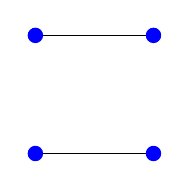
\begin{tikzpicture}[scale=1.5]\label{fig:O(1)}
            \draw (0,0)--(1,0); 
            \draw (0,1)--(1,1);
            \draw[blue,fill=blue] (0,0) circle (0.4ex);
            \draw[blue,fill=blue] (0,1) circle (0.4ex);
            \draw[blue,fill=blue] (1,0) circle (0.4ex);
            \draw[blue,fill=blue] (1,1) circle (0.4ex);
        \end{tikzpicture}
        \caption{Three point function with dressed vertex}
    \end{wrapfigure}
    
        $O(1)$ diagrams only consist of two propagators connecting two external points each. There are three permutations of the diagram which arises by changing position labels. So we have 
        \begin{multline}
            \frac{1}{(x_{12}^2x_{34}^2)^{\Delta}} + \frac{1}{(x_{14}^2x_{23}^2)^{\Delta}} + \frac{1}{(x_{13}^2x_{24}^2)^{\Delta}} = \frac{1}{(x_{12}^2x_{34}^2)^{\Delta}}\\\left(1+\frac{(x_{12}^2x_{34}^2)^{\Delta}}{(x_{14}^2x_{23}^2)^{\Delta}}
            +\frac{(x_{12}^2x_{34}^2)^{\Delta}}{(x_{13}^2x_{24}^2)^{\Delta}} \right)
        \end{multline} 
        Using the crossratio $u = z\bar{z} = \frac{x_{12}^2x_{34}^2}{x_{13}^2x_{24}^2}$ and $v = (1-z)(1-\bar{z})= \frac{x_{14}^2x_{23}^2}{x_{13}^2x_{24}^2}$ we obtain $\frac{1}{(x_{12}^2x_{34}^2)^{\Delta}}\left(1+u^{\Delta}+(\frac{u}{v})^{\Delta}\right)$.
    \subsection{$O(g^2)$ Calculations}
    \begin{figure}[h]
        \centering
        \subfloat[$O(g^2)$ ]{
        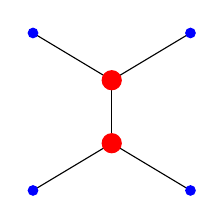
\begin{tikzpicture}[scale=2]\label{fig:O(2)}
            \draw (0,0)--(0.5,0.3); 
            \draw (0.5,0.3)--(1,0);
            \draw (0.5,0.7)--(0,1);
            \draw (0.5,0.3)--(0.5,0.7);
            \draw (0.5,0.7)--(1,1);
            \draw[blue,fill=blue] (0,0) circle (0.2ex);
            \draw[blue,fill=blue] (0,1) circle (0.2ex);
            \draw[blue,fill=blue] (1,0) circle (0.2ex);
            \draw[blue,fill=blue] (1,1) circle (0.2ex);
            \draw[red,fill=red] (0.5,0.7) circle (0.4ex);
            \draw[red,fill=red] (0.5,0.3) circle (0.4ex);
        \end{tikzpicture}}
        \qquad
        \subfloat[$O(g^4)$]{
        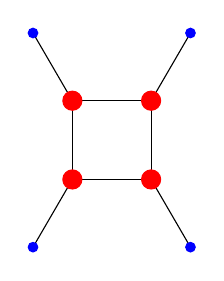
\begin{tikzpicture}[scale=1]\label{fig:O(4)}
            \draw (0,0)--(1,0); 
            \draw (1,1)--(1,0);
            \draw (0,0)--(0,1);
            \draw (1,1)--(0,1);
            \draw (0,0)--(-0.5,-0.86);
            \draw (0,1)--(-0.5,1.86);
            \draw (1,0)--(1.5,-0.86);
            \draw (1,1)--(1.5,1.86);
            \draw[red,fill=red] (0,0) circle (0.8ex);
            \draw[red,fill=red] (0,1) circle (0.8ex);
            \draw[red,fill=red] (1,0) circle (0.8ex);
            \draw[red,fill=red] (1,1) circle (0.8ex);
            \draw[blue,fill=blue] (-0.5,1.86) circle (0.4ex);
            \draw[blue,fill=blue] (-0.5,-0.86) circle (0.4ex);
            \draw[blue,fill=blue] (1.5,-0.86) circle (0.4ex);
            \draw[blue,fill=blue] (1.5,1.86) circle (0.4ex);
    \end{tikzpicture}}
        \caption{Skeleton diagrams for four point function}
    \end{figure}
        Consider the second order diagram ~\ref{fig:O(2)} with two vertices. It is easy to write down the expression corresponding to the diagram. For each propagator, we have a power of $-2\Delta$ over the distance and for every vertex, we have the vertex function calculated in \ref{vertex}. For the case $\Delta_{i} = \Delta \forall i$ we have $\Delta_{ij,k} = \Delta$ and therefore we have 
        
        \begin{equation}
            g^{2}_{\phi\phi\phi}\int\frac{d^{d}x_{5}... d^{d}x_{10}}{\underbrace{(x^{2}_{15}x^{2}_{27}x^{2}_{36}x^{2}_{49})^{\Delta}(x^{2}_{810}}_{propagator})^{\Delta}(\underbrace{x^{2}_{57}x^{2}_{58}x^{2}_{78}}_{vertex 1}\underbrace{x^{2}_{69}x^{2}_{610}x^{2}_{910}}_{vertex 2})^{\frac{d-\Delta}{2}}}
        \end{equation}
        This expreesion can be simplified by using star-triangle formula. Applying the formula five times we finally obtain the expression(Calculations shown in the mathematica file)
        \begin{equation}
            \frac{C_{\phi\phi\phi}^2\Gamma(\Delta)\Gamma(\frac{d-\Delta}{2})}{\pi^{\frac{d}{2}}\Gamma^{2}(\frac{\Delta}{2})\Gamma(\frac{d-2\Delta}{2})}\frac{1}{x_{12}^{3\Delta-d}x_{34}^{\Delta}}\int \frac{d^{d}x_{5}}{x_{15}^{d-\Delta}x_{25}^{d-\Delta}x_{35}^{\Delta}x_{45}^{\Delta}} 
        \end{equation} 
        Star-triangle formula cannot be used further. Although we can write the integral in terms of $\bar{D}$ function defined by
        \begin{equation}\label{def:Dfunction}
            \int \frac{d^{d}y}{\prod_{i=1}^{4}(x_i - y)^{2\Delta_i}} = \frac{\pi^{\frac{d}{2}}}{\prod_{i=1}^{4}\Gamma(\Delta_i)} \frac{x_{14}^{2(h-\Delta_1-\Delta_4)}x_{34}^{2(h-\Delta_3-\Delta_4)}}{x_{13}^{2(h-\Delta_4)}x_{24}^{2\Delta_2}} \bar{D}_{\Delta_1\Delta_2\Delta_3\Delta_4}(u,v)
        \end{equation}
        where $h = \frac{d}{2}$. For the present case we obtain the function $ u^{\frac{d-\Delta}{2}}\bar{D}_{\frac{d-\Delta}{2}\frac{d-\Delta}{2},\frac{\Delta}{2}\frac{\Delta}{2}} (:= f_1(u,v))$. Simillarly one can also calculate the other permutations.
        \begin{align}\label{firstorder}
            f_2(u,v) &= u^{\Delta}v^{\frac{d-3\Delta}{2}} \bar{D}_{\frac{\Delta}{2}\frac{d-\Delta}{2}\frac{d-\Delta}{2}\frac{\Delta}{2}}\\
            f_3(u,v) &= u^{\Delta}\bar{D}_{\frac{\Delta}{2}\frac{d-\Delta}{2}\frac{\Delta}{2}\frac{d-\Delta}{2}} 
        \end{align}
        Combining all these terms we get the first-loop correction to the four-point function
        \begin{equation}\label{firstorderine}
            \frac{C_{\phi\phi\phi}^{2}\Gamma(\Delta)}{\Gamma^{4}(\frac{\Delta}{2})\Gamma(\frac{d-2\Delta}{2})}\left(f_1(u,v)+f_2(u,v)+f_3(u,v) \right)
        \end{equation}
        These $\bar{D}$ functions can be calculated from the following identities.
        \begin{align}\label{Dfunctionidentities}
            \bar{D}_{\Delta_1,\Delta_2,\Delta_3,\Delta_4}(u,v) &= H(\Delta_2,\Sigma-\Delta_4,\Delta_1+\Delta_2-\Sigma+1,\Delta_1+\Delta_2;u,v)\nonumber\\
            H(\alpha,\beta,\gamma,\delta;u,v) &= \frac{\Gamma(1-\gamma)}{\Gamma(\delta)}\Gamma(\alpha)\Gamma(\beta)\Gamma(\delta-\alpha)\Gamma(\delta-\beta)G(\alpha,\beta,\gamma,\delta;u,1-v) \nonumber\\ + \frac{\Gamma(\gamma-1)}{\Gamma(\delta-2\gamma+2)}&\Gamma(\alpha-\gamma+1)\Gamma(\beta-\gamma+1)\Gamma(\delta-\gamma-\alpha+1)\Gamma(\delta-\gamma-\beta+1)\nonumber\\ &\times u^{1-\gamma}G(\alpha-\gamma+1,\beta-\gamma+1,2-\gamma,\delta-2\gamma+2;u,1-v)\nonumber\\
            G(\alpha,\beta,\gamma,\delta;u,1-v) &= \sum_{m,n=0}\frac{(\delta-\alpha)_m (\delta-\beta)_m}{m!(\gamma)_m}\frac{(\alpha)_{m+n}(\beta)_{m+n}}{n!(\delta)_{2m+n}}u^{m}(1-v)^{n}
        \end{align}
        % \\This function can be obtained using properties of $\bar{D}$ function (see appendix for detail). Finally we obtain 
        % \begin{equation}
        %     \bar{D}_{2211}(z,\bar{z}) = -\frac{(2-z-\bar{z})\phi^{(1)}(z,\bar{z})}{(z-\bar{z})^3} - \frac{\frac{ln v(z+\bar{z}-2u)}{u} + 2ln u}{(z-\bar{z})^2}
        % \end{equation} 
    \subsection{$O(g^4)$ Calculations}
        Fourth order calculation is also similar to the previous calculation. We have the diagram\ref{fig:O(4)} which translate to
        \footnotesize
        \begin{equation}
            g_{\phi\phi\phi}^{4}\int \frac{d^{d}x_5\cdots d^{d}x_{16}}{(x_{15}x_{26}x_{37}x_{48}x_{1011}x_{1213}x_{1415}x_{169})^{2\Delta}(\underbrace{x_{59}x_{510}x_{910}}_{Vertex 1}\underbrace{x_{611}x_{612}x_{1112}}_{Vertex 2}\underbrace{x_{713}x_{714}x_{1314}}_{Vertex 3}\underbrace{x_{815}x_{816}x_{1516}}_{Vertex 4})^{d-\Delta}}
        \end{equation}
        \normalsize
        Again applying star-triangle formula couple of times we finally obtain the equation
        \begin{equation}
           \frac{C_{\phi\phi\phi}^{4}\Gamma^{4}(\Delta)\Gamma^8(\frac{d-\Delta}{2})}{\pi^{2d}\Gamma^8(\frac{\Delta}{2})\Gamma^4(\frac{d-2\Delta}{2})} \int \frac{d^{d}x_5d^{d}x_6d^{d}x_7d^{d}x_8}{(x_{15}x_{26}x_{37}x_{48})^{3\Delta-d}(x_{28}x_{25}x_{36}x_{47}x_{56}x_{67}x_{78}x_{58})^{d-\Delta}}
        \end{equation}
        This equation cannot be further simplified for general dimension and $\Delta$. But the complexity reduces if we take $d=6$ and $\Delta = 2$. Four terms then just dropped. Now we can use star-triangle formula few more times to finally obtain 
        \begin{equation}
            \frac{h(z,\bar{z})}{(x_{13}^2x_{24}^2)^{\Delta_{\phi}}} = C_{\phi\phi\phi}^4 \int \frac{d^{d}x_5d^{d}x_7}{\pi^6} \frac{1}{x_{15}^2x_{35}^2x_{17}^2x_{37}^2(x_{57}^2x_{25}^2x_{47}^2)^2}
        \end{equation}
        % It was shown in the appendix of the paper \ref{vasco} that this integral satisfies a differential equation from which one can extract the final answer.
        where explicit position dependence has been pulled out to obtain a function $h(z,\bar{z})$ depending solely on the conformally invariant cross-ratios or equivalently on $z$ and $\bar{z}$. Further integration is difficult but one can obtain a differential equation satisfied by the above equation. For that we will let the Laplacian on co-ordinate $x_2$ act on both the side. In the left hand side Laplacian can be transformed into $(z,\bar{z})$ co-ordinate to obtain
        \begin{equation}
            4\left[\partial_z\partial_{\bar{z}} - 2\frac{\partial_z - \partial_{\bar{z}}}{z-\bar{z}}\right]h(z,\bar{z})
        \end{equation} 
        while for the right hand side we can use the identity $\nabla_2^2 \frac{1}{(x_2^2)^2} = -4\pi^3\delta^6(x_2)$ and perform $x_5$ integral
        \begin{equation}
            -4 \int \frac{d^6x_7}{\pi^3} \frac{1}{x_{12}^2x_{23}^2x_{17}^2x_{37}^2(x_{27}^2x_{47}^2)^2}
        \end{equation} 
        The integral can be identified with $\bar{D}$ function. Writing everything in terms of the cross ratios we get
        \begin{equation}
            uv\left[\partial_z\partial_{\bar{z}} - 2\frac{\partial_z - \partial_{\bar{z}}}{z-\bar{z}}\right]h(z,\bar{z}) = -\bar{D}_{1212}(z,\bar{z})
        \end{equation}
        Using identities from \cite{dfunction} and writing $h(z,\bar{z})$ in terms of another function we get the following relation
        \begin{equation}
            uv*\Delta\left(\frac{u}{v}\partial_u + \partial_v\right)v\frac{f(z,\bar{z})}{z-\bar{z}} = \left(\frac{u}{v}\partial_u + \partial_v\right)\frac{uv}{z-\bar{z}}\partial_z\partial_{\bar{z}}f(z,\bar{z}) = -\left(\frac{u}{v}\partial_u + \partial_v\right) v \bar{D}_{1111}
        \end{equation}
        where $\Delta = \partial_z\partial_{\bar{z}} - 2\frac{\partial_z - \partial_{\bar{z}}}{z-\bar{z}}$. So we get simpler differential equation
        \begin{equation}
            u\partial_z\partial_{\bar{z}}f(z,\bar{z}) = -\phi^{(1)}(z,\bar{z})
        \end{equation}
        This equation is satisfied by $\phi^{(2)}(z/(z-1,\bar{z}/(\bar{z}-1)))$. So finally we obtain 
        \begin{equation}
            h(z,\bar{z}) = - \left(\frac{u}{v}\partial_u + \partial_v\right)\frac{v}{z-\bar{z}}\phi^{(2)}(z/(z-1,\bar{z}/(\bar{z}-1)))
        \end{equation}
        Rest of the permutations can be found just by changing the variable $(z \to z^{-1},\bar{z}\to\bar{z}^{-1} )$ and $(z\to\frac{z}{z-1},\bar{z}\to\frac{\bar{z}}{\bar{z}-1})$. Finally ,we get the second-loop correction
        \begin{equation}
            C_{\phi\phi\phi}^4\left(u^2h(z,\bar{z}) + h(z^{-1},\bar{z}^{-1}) + \left(\frac{u}{v}\right)^2h\left(\frac{z}{z-1},\frac{\bar{z}}{\bar{z}-1} \right) \right)
        \end{equation}

\chapter{Conformal Block Decomposition}\label{conformal-block-decomposition}
    \section{Operator Product Expansion}
    Suppose two operators are inserted inside a sphere to produce a state $|\psi\rangle$ on the sphere. Now the Hilbert space being separable we can decompose the state into countable basis element. For example we can write the state in terms of energy eigenstates $|\psi\rangle = \sum_{n}c_{n}|E_{n}\rangle$. Now by state-operator correspondence, each energy eigenstates are in relation with either primaries or their descendants. This can compactly be written as a sum over all primaries and encoding the descendants in a differential prefactor $C_{\mathcal{O}}(x,\partial_x)$.
    \begin{equation}
        \phi_1(x)\phi_2(0)|0\rangle = |\psi\rangle = \sum_{\mathcal{O} primaries} C_{\mathcal{O}}(x,\partial_y)\mathcal{O}(y)|_{y=0}|0\rangle
    \end{equation}  
    In Quantum mechanics or in QFT we cannot proceed further without given any information about the specifics of the operators inserted and the energy eigenstates. But Conformal symmetry in the system forces tight constraints which makes us able to figure out these prefactors upto some coefficients known as OPE coefficients. 
    \begin{equation}
        \phi_1(x)\phi_2(0) = \sum_{\mathcal{O}} \lambda_{12\mathcal{O}}\mathcal{C}_{\mathcal{O}}(x,\partial_y)\mathcal{O}(y)|_{y=0}
    \end{equation}
    To sketch out how to obtain these $\mathcal{C}_{\mathcal{O}}(x,\partial_y)$ we insert a operator into two point function and compute the three point function using OPE expansion.
    \begin{align}
        \langle\phi_1(x)\phi_2(0)\Phi(z)\rangle &= \sum_{\mathcal{O}} \lambda_{12\mathcal{O}}\mathcal{C}_{\mathcal{O}}(x,\partial_y)\langle\mathcal{O}(y)|_{y=0}|\Phi(z)\rangle\\
        &= \lambda_{12\Phi}\mathcal{C}_{\Phi}(x,\partial_y)\langle\Phi(y)|\Phi(z)\rangle\\
        \frac{C_{12\Phi}}{x^{\Delta_{12,\Phi}}z^{\Delta_{2\Phi,1}}|x-z|^{\Delta_{1\Phi,2}}} &= \lambda_{12\Phi}\mathcal{C}_{\Phi}(x,\partial_y) \left(\frac{1}{|y-z|^{2\Delta_{\Phi}}}\right)
    \end{align}
    where we have used the orthonormality of the state in the second line and the form of two-point and three-point functions in the last line. In the last equation if we expand both sides in small x and match the coefficients we can fix the form of $\mathcal{C}_{\mathcal{O}}(x,\partial_y)$.
% \documentclass[a4paper]{report}
%     \usepackage[utf8]{inputenc}
%     \usepackage[english]{babel}
%     \usepackage{amsmath}
%     \usepackage{amssymb}
%     \usepackage{amsthm}
%     \usepackage{graphicx}
%     \usepackage{hyperref}
%     \usepackage[top=1in, bottom=1.25in, left=1in, right=1in]{geometry}
%     \usepackage{wrapfig}
%     \theoremstyle{definition}
%     \newtheorem{definition}{Definition}[section]
%     % \theoremstyle{remark}
%     % \newtheorem*{remark}{Remark}
%     % \newtheorem*{theorem}{Theorem}
%     \usepackage[autostyle]{csquotes}
%     \usepackage{float}
%     \usepackage[font={small,it}]{caption}
%     \usepackage[title]{appendix}
%     \usepackage{subfig}
%     \usepackage[export]{adjustbox}
%     \usepackage{tikz}
%     \title{A note on the paper Skeleton expansion and large spin bootstrap for $\phi^3$ theory\ref{vasco}}
%     \author{Biplab Mahato}
%     \begin{document}
        \section{Conformal Blocks}
            Consider the four point function. We can use the OPE expansion for two pairs of fields toget
            \begin{equation}\label{12decomposition}
                \langle\phi(x_1)\phi(x_2)\phi(x_3)\phi(x_4)\rangle = \sum_{\mathcal{O}}\lambda_{12\mathcal{O}}\lambda_{34\mathcal{O}}\left(\mathcal{C}_{\mathcal{O}}(x_{12},\partial_y)\mathcal{C}_{\mathcal{O}}(x_{34},\partial_z)\langle\mathcal{O}(y)\mathcal{O}(z) \rangle \right)
            \end{equation}
            where the expreesion in the bracket is completely determined by the conformal invariance. These are called conformal partial waves or the conformal blocks. The coefficients on the other hand is known as OPE coefficients. One can easily factor out the position dependence from the four point function and be left with a function solely dependent on the two conformally invariant cross-ratios. 
            \begin{equation}
                \langle\phi(x_1)\phi(x_2)\phi(x_3)\phi(x_4)\rangle = \frac{\mathcal{A}(u,v)}{(x_{12}^2x_{34}^2)^{\Delta_{\phi}}}
            \end{equation} 
            the function $\mathcal{A}(u,v)$ can now be written in terms of conformal blocks
            \begin{equation}
                \mathcal{A}(u,v) = 1 + \sum_{\mathcal{O}}\lambda_{12\mathcal{O}}\lambda_{34\mathcal{O}}G_{\mathcal{O}}(u,v)
            \end{equation}
            where the function $G_{\mathcal{O}}(u,v)$ is known for all dimensions(closed forms are only known for even dimensions)(note that 1 is coming from the identity operator). \\
            An operator is characterised by its dimension and its spin. So the sum over primaries can be replaced by the sum over dimensions and spins. Spins can take only half integer values (in this case only integer values are allowed as free scalar field describe bosons). Conformal block for generic values of scaling dimension and spin are given by
            \begin{equation}\label{uvexpansionofblock}
                G_{\Delta,l}^{d}(u,v) = \sum_{m=0}^{\infty} u^{\frac{\Delta-l}{2}+m} g_{m,l}(v)
            \end{equation}
            where $g_{m,l}(u,v)$ satisfy the differential equation\cite{regge}
            \footnotesize
            \begin{multline}
                4v(v-1)^2g_{m,l}''(v) - 2(v-1)g_{m,l}'(v)\left(2v(-\Delta+l-2m-1)\right) \\+ g_{m,l}(v)(4m(-d+mv+m)+l^2(v-1)-2l(\Delta+2m(v+1)+\Delta v -2) + 4\Delta m(v+1)+\Delta^2(v-1) ) \\= 4v(v+1)g_{m-1,l}''(v)+ 2g_{m-1,l}'(v)\left(2v(\Delta-l+2m-1)+2 \right) + g_{m-1,l}\left(-\Delta+l-2m+2 \right)\left(-\Delta+l-2m+2 \right)
            \end{multline}
            \normalsize
            for the purpose of this text we only need the first two of these
            \begin{eqnarray}\label{g0g1}
                g_{0,l}(u,v) &=& \left(\frac{v-1}{2}\right)^{l} {}_2F_1\left(\frac{\Delta+l}{2},\frac{\Delta+l}{2};\Delta+l;1-v\right)\\
                g_{1,l}(u,v) &=& \frac{\Delta(l+\Delta)^2(\Delta-1)}{(\Delta+l-1)(\Delta+l+1)(\Delta+1-\frac{d}{2})} {}_2F_1\left(\frac{\Delta+2}{2},\frac{\Delta+2}{2};\Delta+2;1-v\right)\nonumber
            \end{eqnarray}
            The expansion of this form is effective while considering low twist ($\tau = \Delta-l$) contributions to the four-point function. The next section provides the details of determining those contributions.
        \section{Conformal Block Decomposition}
            To get an idea how the OPE co-efficients are fixed we will go through the process of conformal block decomposition for the tree level. Higher order calculations will be sketched.
            \subsection{Tree-level}
                First consider the tree-level four-point function.
                \begin{equation}
                    \mathcal{A}(u,v) = 1 + u^{2} + \left    (\frac{u}{v}\right)^{2} + O(\epsilon)
                \end{equation}
                We will try to match the this with the  conformal waves in the OPE limit ($z\to 0,   \bar{z}\to0 $ or $u\to 0,v\to 1$). So we   will write everything in terms of $u$ and a   new variable $x = (1-v)$. The four-point  function becomes.
                \begin{eqnarray}
                    \mathcal{A}(u,x) = 1 + u^2 + u^2\sum_   {n=0}^{\infty} n x^n
                \end{eqnarray}
                First term can be matched with the identity.    Rest of the terms has a commom factor of   $u^2$. It is clear that we must have  $\Delta-l = 4$ with $m=0$ so that we have $G_    {4+l,l}^{6}(u,v) = u^2 g_{0,l}(v)$. So now  it boils down to the equation 
                \begin{equation}
                    \sum_{n=0}^{\infty} n x^n = \sum_{l=0 \\    even}^{\infty} p_{0,l} g_{0,l}(1-x) 
                \end{equation}
                This equation at first glance seems daunting    to solve for $p_{0,l}$. But notice the     factor $x^l$ in front of Hypergeometric     function. Hypergeometric function near $x=0$    behaves like a power series with no    divergence. So overall $g_{0,l}$ starts    contributing after $x^l$. This reduces the     infinite sum to finite for each co-efficient    of some power of x. Comparing co-efficients    on both side now it become easy to solve for   $p_{0,l}$. The values have a closed form  formula which can be found in    Mathematica\footnote{Using the command     \textit{FindSequenceFunction} in Mathematica}   .
                \begin{equation}
                    p_{0,l} = \frac{2^l (l+2)!(l+1)! }{(2l+1)!}   
                \end{equation} 
            \subsection{First order calculations}
                In first order in $\epsilon$, $\bar{D}$ functions in \ref{firstorderine} will start contributing. Note that there is not any $u^0$ term. Contribution starts from $u^1$. This is expected as unitary bound\footnote{We are treating $\phi^3$ theory as a perturbation to the free theory, so we can use the unitary bounds for the free theory even though $\phi^3$ theory is not unitary for real coupling constant} (\ref{unitary}) constraints $\Delta\geq\frac{6-2}{2}=2$ for scalar operator and twist $\tau = \Delta-l\geq6-2=4$. And on the right hand side conformal blocks have $u^{\frac{\tau}{2}}$ character. So $u^0$ term is not allowed in the theory. Also it is clear that $u^1$ terms will be matched by only the scalar operator saturating the unitary bound. Note that this scalar operator is the operator $\phi$.\\
                Among the three permutaions of order $\epsilon$ terms only one $(f_1)$ have $u^1$ term (as $\bar{D}_{2,2,1,1}(u,v)$ has a factor of $1/u$). So we must have \footnote{note that $C_{\phi\phi\phi}^2\approx\epsilon+O(\epsilon^2)$ so at order $\epsilon$ we should take only the leading terms in d and $\Delta$}
                \begin{equation}
                    \frac{C_{\phi\phi\phi}^{2}\Gamma(\Delta)}{\Gamma^{4}(\frac{\Delta}{2})\Gamma(\frac{d-2\Delta}{2})}f_1(u,v) = C_{\phi\phi\phi}^2u{}_2F_1\left(1,1,2,1-v \right)
                \end{equation}
                Two sides matches exactly without giving any constraints!\\
                At order $u^2$ two kind of terms arises; one with log(u) factor and one without it. $log(u)$ factor arises from the anomalous dimensions in conformal partial waves ($u^{\frac{\tau}{2}} = u^{2+\frac{1}{2}\epsilon \gamma_l^{(1)}} = u^2(1+\frac{1}{2}\epsilon\gamma_l^{(1)}log(u))$). By matching co-eeficient on both side we get the expression 
                \begin{equation}
                    \gamma_l^{(1)} = \frac{4}{3(l+1)(l+2)}
                \end{equation} 
                Using this expression if we try to match without log terms at the same order we will get the first order corrections to the ope co-efficients.
                \begin{align}
                    p_{0,l} &= \frac{2^l (l+2)!(l+1)! }{(2l+1)!}(1+\epsilon\mathcal{P}_l + \epsilon^2Q_l)\nonumber\\
                    \text{where } \mathcal{P}_l &= -\frac{4(7+5l(3+l))S_l}{9(l+1)(l+2)} + \frac{2(4+5l(3+l))S_{2l}}{9(l+1)(l+2)}-\frac{6-5l(1+l)(4l^2+6l-1)}{9(1+l)^2(2+l)(1+2l)}
                \end{align}
                Also at this order first order corrections to $\Delta_{\phi}$ along with $C_{\phi\phi\phi}^2$ is fixed: $\Delta_{\phi} = \frac{d-2}{2}-\frac{\epsilon}{18}+O(\epsilon^2)$ and $C_{\phi\phi\phi}^2 = -\frac{2}{3}\epsilon + O(\epsilon^2)$. Negative OPE coefficients for the scalar function implies that that theory in fixed point is not unitary.
            \subsection{Second order calculations}  
             At second order in epsilon calculation goes similar to the first order. 
             \begin{itemize}
                 \item order $u^1$ is matched by scalar part of the conformal block.
                 \item at $u^2$, $log^2(u)$ and $log(u)$ terms gives the second order corrections to the anomalous dimension.
                 \begin{equation}
                     \gamma_l^{(2)} = \frac{2(86-l(-177+l(382+l(492+127l))))}{243(1+l)^3(2+l)^3} + \frac{20S_l}{27(1+l)(2+l)}
                 \end{equation}
                 \item at $u^2$ regular terms gives the second order corrections to OPE coefficients.
                 \begin{multline}
                    Q_2 = -\tfrac{26591}{1749600}, Q_4 = \tfrac{61563941}{267907500},Q_6 = \tfrac{2047344914778847}{4123293433459200},Q_8 = \tfrac{349552895612696393}{455981556990960000},\\Q_{10} = \tfrac{1368755978809447171291}{1327848692728141584000}
                \end{multline}
                \item finally, the  corrections to the scalar operator
                \begin{equation}
                    \Delta_{\phi} = \frac{d-2}{2}-\frac{\epsilon}{18}-\frac{43}{1458}\epsilon^2 + O(\epsilon^3);\hspace{10pt}C_{\phi\phi\phi}^2 = - \frac{2}{3}\epsilon-\frac{143}{243}\epsilon^2 + O(\epsilon^3)
                \end{equation}
             \end{itemize}
        
    % \end{document}
% \chapter{Large Spin Bootstrap}
    % \section{Conformal Bootstrap}
    % Recall the OPE expansion of the four-point function in \ref{12decomposition}. There we made a choice of 'contracting' (12) and (34). Other choices are equally good and in principle should spits out the same answer at the end. This realisation gives rise to the concept of conformal bootstap. Consider expanding in the (14) and (23) channel. This corresponds to the replacement ($u\to v, v\to u$). So we do not have to re-calculate $\mathcal{A}(u,v)$. The replacement will produce the desired function. So by consistency relation we have.
    % \begin{equation}
    %     \frac{\mathcal{A}(u,v)}{(x_{12}^2x_{34}^2)^{\Delta_{\phi}}} = \frac{\mathcal{A}(v,u)}{(x_{14}^2x_{23}^2)^{\Delta_{\phi}}}
    % \end{equation} 
%     This equation can be recasted as follows
%     \begin{eqnarray}
%         \left(1+\sum_{\mathcal{O}} \lambda_{\mathcal{O}}^{2}G_{\mathcal{O}}(u,v)\right) = \left(\frac{u}{v}\right)^{\Delta_{\phi}} \left(1+\sum_{\mathcal{O}} \lambda_{\mathcal{O}}^{2}G_{\mathcal{O}}(v,u)\right)\\
%         1 = \sum_{\mathcal{O}}\lambda_{\Delta_{\phi}} \left[\frac{v^{\Delta_{\phi}}G_{\mathcal{O}}(u,v) - u^{\Delta_{\phi}}G_{\mathcal{O}}(v,u)}{u^{\Delta_{\phi}}-v^{\Delta_{\phi}}}\right]
%     \end{eqnarray}
%     where we have used the compact notation for the OPE as $\lambda_{\mathcal{O}}^{2}$. The square reflecting the fact that OPE co-efficients are all non-negative. 

\chapter{Inversion Integral}\label{inversion-integral}
\section{Conformal Bootstrap}
    Recall the OPE expansion of the four-point function in \ref{12decomposition}. There we made a choice of 'contracting' (12) and (34). Other choices are equally good and in principle should spit out the same answer at the end. This realisation gives rise to the concept of conformal bootstap. Consider expanding in the (14) and (23) channel. This corresponds to the replacement ($u\to v, v\to u$). So we do not have to re-calculate $\mathcal{A}(u,v)$. The replacement will produce the desired function. So by consistency relation we have.
    \begin{align}
        \frac{\mathcal{A}(u,v)}{(x_{12}^2x_{34}^2)^{\Delta_{\phi}}} &= \frac{\mathcal{A}(v,u)}{(x_{14}^2x_{23}^2)^{\Delta_{\phi}}}\nonumber\\
        \text{or, }\mathcal{A}(u,v) &= \left(\frac{u}{v}\right)^{\Delta_{\phi}}\mathcal{A}(v,u)
    \end{align}
    This equation is known as Bootstrap equation. In terms of conformal blocks one then can write
    \begin{equation}\label{conformalbootstrapequation}
        \sum_{\mathcal{O}_k}C_{\phi\phi\mathcal{O}_k}^2G_{\Delta_k,l_k}(u,v) = \left(\frac{u}{v}\right)^{\Delta_{\phi}}\sum_{\mathcal{O}_k}C_{\phi\phi\mathcal{O}_k}^2G_{\Delta_k,l_k}(v,u)
    \end{equation}
    We will be focusing on the limit $u\to0$, $v\to0$. From \ref{uvexpansionofblock} and \ref{g0g1} we can see that the left hand side diverges as log(v) while the right hand side have a power law divergence. To fix this mismatch in singularities we must sum up infinite tower of operators having different spin but same twist. To generate the power law singularity contributions should come from the tail of the sum. This motivates the idea of expansion in large spin i.e. expanding in inverse power of conformal spin $\frac{1}{J^2}$ where $J^2 = (2l+\tau)(2l+\tau-2)$. Large spin bootstrap has been used to calculate anomalous dimensions and OPE coefficients upto order $\epsilon$ in \cite{largespinbootstrap}. At $\epsilon^2$, calculation becomes complicated. A simpler method to obtain CFT data is given in \cite{inversiongravitation}where an integral formula is derived to obtain CFT data from the nature of discontinuties in the right hand side of \ref{conformalbootstrapequation}.
   \section{Inversion Formula}
        It is more convinient to work in the $(z,\bar{z}$) coordinates and a different normalisation of conformal blocks. Consider the conformal blocks $f_{\Delta,l}(\bar{z})$ \footnote{We are working at small z limit where only the lowest order in z is kept. Dependence on the z variable is suppressed to remind that we have taken $z\to0$} where,
        \begin{equation}
            f_{\Delta,l}(\bar{z}) = r_{\frac{\Delta+l}{2}}k_{\frac{\Delta+l}{2}}(\bar{z})
        \end{equation} 
        with $r_h = \frac{\Gamma(h)^2}{\Gamma(2h)}$ and $k_h(\bar{z}) = \bar{z}^h{}_2F_1(h,h,2h,\bar{z})$. We want to calculate the constants $\hat{a}_l$ such that
        \begin{equation}
            \sum_{\Delta = 2\Delta_{\phi}+l,\\l=0,2,\cdots} \hat{a}_lf_{\Delta,l}(\bar{z}) = \mathcal{A}(\bar{z})
        \end{equation}
        As discussed in \cite{inversiongravitation} and \cite{taming} $\mathcal{A}(\bar{z})$ has an enhanced singularity at $\bar{z}\to1$. This singularity alone carry the informations about the OPEs and anomalous dimensions. As derived in \cite{inversiongravitation} $\hat{a}$ can be calculated using the following inversion formula
        \begin{equation}
            \hat{a}(\bar{h}) = \frac{2\bar{h}-1}{\pi^2}\int_0^1dtd\bar{z}\frac{\bar{z}^{\bar{h}-2}(t(1-t))^{\bar{h}-1}}{(1-t\bar{z})^{\bar{h}}}\text{dDisc}[\mathcal{A}(\bar{z})]
        \end{equation}
        Following sections explain the above equation as well as how to extract anomalous dimensions and OPE coefficients  from it.
    \subsection{Double Discontinuity}
        Double discontinuity of a complex function is defined to be
        \begin{equation}
            \text{dDisc}[f(z)] = f(z) - \frac{1}{2}\left(f^{\circlearrowleft}(z) + f^{\circlearrowright}(z) \right)
        \end{equation}
        where $f^{\circlearrowleft,\circlearrowright}(z)$ is the clockwise and counter-clockwise analytic continuation around the branch-point. Following examples will illustrate how to calculate double discontinuity of some common functions.
        \subsubsection*{f(z) = z$^p$}
            In polar coordinate a point can be written as $z = re^{i\theta}$. Where $\theta$ is the argument of $z$. This $\theta$ is not uniquely defined as the transformation $\theta\to\theta+2n\pi, n\in\mathbb{Z}$ does not give a new point. For analytic function, this transformation leaves also the function invariant. Another class of function which does not respect the transformation but when restricted to any $2\pi$ interval for $\theta$ behave like analytic functions. Branch points and branch cuts are introduced to deal with these multi-valued functions. Take the example of the function $f(z) = z^p = r^pe^{ip\theta}$. Going around the origin(counterclockwise) and reaching the same point the function becomes $r^pe^{ip\theta}e^{2ip\pi}$ i.e. picks up a phase factor of $e^{2ip\pi}$. The phase factors vanish for integer values of $p$. For other values of $p$, this function becomes a multivalued function. Introducing a branch cut say a line from the origin to infinity along the x-axis($\theta=0$) and staying in one branch (without crossing the cut) produce an analytic function on the whole plane except at the branch cut. Other branches will have the phase factor associated to it.\par
            After the above discussion following definitions are obvious
            \begin{equation}
                f^{\circlearrowleft}(z) = f(ze^{2i\pi}); \hspace{5pt} f^{\circlearrowright}(z) = f(ze^{-2i\pi})
            \end{equation} 
            Now it is easy to calculate the double discontinuity
            \begin{eqnarray}
                dDisc[z^p] &=& z^p-\frac{1}{2}z^p(e^{2ip\pi}+e^{-2ip\pi})\nonumber\\
                &=& z^p(1-cos(2p\pi)) = 2sin^2(p\pi)z^p
            \end{eqnarray} 
        \subsubsection*{f(z) = log(z)}
            \begin{equation}
                dDisc[log(z)] = log(z) - \frac{1}{2}((log(z)+2i\pi)+(log(z)-2i\pi)) = 0
            \end{equation}
            i.e. log(z) does not have any double discontinuity.
        \subsubsection*{f(z) = log$^2$(z)}
            \begin{eqnarray}
                dDisc[log^2(z)] &=& log^2(z) - \frac{1}{2}((log(z)+2i\pi)^2+(log(z)-2i\pi)^2)\nonumber\\
                &=& log^2(z)-\frac{1}{2}(log^2(z)+4i\pi log(z)-4\pi^2+log^2(z)-4i\pi log(z)-4\pi^2)\nonumber\\
                &=& 4\pi^2
            \end{eqnarray}
    \subsection{Integral}\label{inversion_integral}
        With closed form expression of double discontinuity in hand, inversion integral can be tackled. For example consider discontinuity of the form $\left(\frac{\bar{z}}{1-\bar{z}}\right)^p$, where we have a pole at $\bar{z} = 1$ for positive values of $p$. The double integral can be separated by changing variable $\bar{z}\to \zeta = \frac{\bar{z}(1-t)}{1-t\bar{z}}$.
        \begin{align}
            \hat{a}(\bar{h}) &= \frac{2(2\bar{h}-1)sin^2(p\pi)}{\pi^2}\int_{0}^{1}dt d\bar{z}\frac{\bar{z}^{\bar{h}-2}(t(1-t))^{\bar{h}-1}}{(1-t\bar{z})^{\bar{h}}} \left(\frac{\bar{z}}{1-\bar{z}}\right)^{p} \nonumber\\
            &= \frac{2(2\bar{h}-1)sin^2(p\pi)}{\pi^2}\int_{0}^{1}dtd\zeta (t^{\bar{h}-1}(1-t)^{-p})(\zeta^{\bar{h}+p-2}(1-\zeta)^{-p})\\
            &= \frac{2(2\bar{h}-1)sin^2(p\pi)}{\pi^2} \frac{\Gamma(\bar{h})\Gamma(1-p)}{\Gamma(\bar{h}-p+1)}\frac{\Gamma(\bar{h}+p-1)\Gamma(1-p)}{\Gamma(\bar{h})}\nonumber\\
            &= \frac{2(2\bar{h}-1)\Gamma(\bar{h}+p-1)}{\Gamma(p)^2\Gamma(\bar{h}-p+1)}\nonumber
        \end{align}
        where the identity $\Gamma(p)\Gamma(1-p) = \frac{\pi}{sin(p\pi)}$ is used in the last line. Note that now we can analytically continue the last formula for all values of $p$. Integral for any other function can be done by first writing the function in powers of $\frac{\bar{z}}{1-\bar{z}}$ then using the above formula for each term and finally summing all the term. This way we obtain the following integrals which will be used later to determine ope data.
        \begin{table}[h]
        \begin{center}
        \begin{tabular}{c|c}
            
            $\mathcal{A}(\bar{z}$) & $\hat{a}(\bar{h})$\\
            \hline\hline
            $log^2(1-\bar{z})$ & $\dfrac{4(2\bar{h}-1)}{\bar{h}(\bar{h}-1)}$\\
            $log^2(1-\bar{z})log(\bar{z})$ & $-\dfrac{4(2\bar{h}-1)}{\bar{h}^2(\bar{h}-1)^2}$\\
        \end{tabular} 
        \end{center}
        \caption{Inversions for $G(\bar{z})$}
        \end{table}
    \subsection{CFT data}
        Once $\hat{a}(\bar{h})$ is calculated for $\mathcal{A}(\bar{z})$ upto necessary order CFT data can be recovered from it by following protocol.
        \begin{itemize}
        \item Remove the overall $z^{\Delta_{\phi}}$ factor.
        \item Individual terms will be accompanied with some power of $log(z)$. Group all those terms with some power(say $k$) of $log(z)$ and call those terms(without the log part) as $\frac{1}{k!2^k}U_{\bar{h}}^{(k)}$.
        \item CFT data are related to the $U_{\bar{h}}$'s as follows
                    \begin{equation}
                        \hat{a}_l(\gamma_l)^k = U_{\bar{h}}^{(k)} + \frac{1}{2}\partial_{\bar{h}}U_{\bar{h}}^{(k+1)} + \frac{1}{8}\partial_{\bar{h}}^2U_{\bar{h}}^{(k+2)} + \cdots
                    \end{equation}
                \item Actual OPE coefficients are related to $\hat{a}_l$ by the relation $a_{\Delta,l} = 2^lr_{\frac{\Delta+l}{2}}\hat{a}_l$ \footnote{$2^l$ factor is coming due to the usage of different normalisation of conformal blocks}, where $r_h = \frac{\Gamma(h)^2}{\Gamma(2h)}$ and $\bar{h} = l+ \Delta_{\phi}$.
            \end{itemize}
    \section{Calculations}
        \subsection{Using Skeleton Expansion}
            To start calculations we first need $\mathcal{A}(\bar{z})$ i.e. small z limit of the four point function. We have already calculated the four point function upto order $O(\epsilon^2)$ in chapter \ref{skeleton}. Small z limit of that can be obtained. But first note that earlier $\bar{D}$ functions are expanded in the limit $u\to0,v\to1$, whereas here we need $u\to0,v\to0$ limit. This limit can be obtained from the Mellin-Barnes representation \cite{mellinbarnes} of $\bar{D}$ function. 
            \begin{align}
                \bar{D}_{\Delta_1,\Delta_2,\Delta_3,\Delta_4}(u,v) &= \frac{1}{2\pi i}\frac{1}{2\pi i}\int_{c-i\infty}^{c+i\infty} \frac{ds}{2}\frac{dt}{2}u^{\tfrac{s}{2}}v^{\tfrac{t}{2}}\Gamma(-\tfrac{s}{2})\Gamma(-\tfrac{s}{2}+\tfrac{\Delta_3+\Delta_4-\Delta_1-\Delta_2}{2})\Gamma(-\tfrac{t}{2})\nonumber\\ &\Gamma(-\tfrac{t}{2}+\tfrac{\Delta_1+\Delta_4-\Delta_2-\Delta_3}{2})\Gamma(\Delta_2+\tfrac{s+t}{2})\Gamma(\tfrac{s+t}{2}+\tfrac{\Delta_1+\Delta_2+\Delta_3-\Delta_4}{2})
            \end{align}
            Where $c>0$. That is, we are supposed to integrate it along a line parallel to imaginary axis. This is usually done by closing the loop on the left and pushing the loop towards infinity. The loop encloses all the poles of gamma function on the negative real axis(integre values). Integral then can be done using Residue theorem. Note that each pole gives different powers of u and v. As we only need small u small v limit, we do not have to evaluate all the residues. We will be interested in the poles $s=-2,0$ and $t=-2,0$. Evaluating these give the desired expansion of $\bar{D}$ function required for the calculations.\par 
            Now that we have the correlator we can start taking the small z limit (keeping an overall factor of $z^2$ ) and picking out the terms having double discontinuity.\par
            Firstly, at tree level (\ref{tree}) only divergent term is $\left(\frac{u}{v}\right)^{\Delta_{\phi}}$. In small z limit this reduces to 
            \begin{equation}
                z^{\Delta_{\phi}}\left(\frac{\bar{z}}{1-\bar{z}} \right)^{\Delta_{\phi}} \xrightarrow{\text{inversion}} \frac{2(2\bar{h}-1)\Gamma(\bar{h}+\Delta_{\phi}-1)}{\Gamma(\Delta_{\phi})^2\Gamma(\bar{h}-\Delta_{\phi}+1)}
            \end{equation}
            This easily translate to the OPE co-efficient as 
            \begin{equation}
                p_{0,l} = \frac{2^l\Gamma(\Delta_{\phi}+l)^2}{\Gamma(2\Delta_{\phi}+2l)}\frac{2(2l+2\Delta_{\phi}-1)\Gamma(l+2\Delta_{\phi}-1)}{\Gamma(\Delta_{\phi})^2\Gamma(l+1)}\to \frac{2^{l+1}\Gamma(d/2+l-1)^2\Gamma(d+l-3)}{l!\Gamma(d+2l-3)\Gamma(d/2-1)^2}
            \end{equation}
            At one loop we have two kinds of double discontinuities. One coming from the $\frac{1}{1-\bar{z}}$ type divergences and other coming from the $log^2(v)$ terms. At two loop only $log^2(1-\bar{z})$ terms are present. We already know from how to obtain the inversion integral of these. From these we collect terms in powers of log(z) identified from the equation $U_{\bar{h}}^{(0)} + \frac{1}{2}log(z)U_{\bar{h}}^{(1)} + \frac{1}{8}log^2(z)U_{\bar{h}}^{(2)}$. From these we can recover the CFT data
            \begin{align}
                U_{\bar{h}}^{(0)} +\frac{1}{2}\partial_{\bar{h}}U_{\bar{h}}^{(1)} + \frac{1}{8}\partial_{\bar{h}}^2U_{\bar{h}}^{(2)}  &= a_l^{(0)} + \epsilon a_l^{(1)} + \epsilon^2a_l^{(2)}\nonumber\\
                U_{\bar{h}}^{(1)} +\frac{1}{2}\partial_{\bar{h}}U_{\bar{h}}^{(2)} &= \epsilon \left(a_l^{(0)}\gamma_l^{(1)}\right) + \epsilon^2\left(a_l^{(0)}\gamma_l^{(2)} + a_l^{(1)}\gamma_l^{(1)} \right)\\
                U_{\bar{h}}^{(2)} &= \epsilon^2\left(a_l^{(0)}(\gamma_l^{(1)})^2\right)\nonumber
            \end{align}
            Recovered data exactly matched the anomalous dimensions and OPEs calculated earlier. 
        \subsection{Using Conformal Bootstrap}
            Conformal bootstrap methods can be used independently to obtain the CFT data without using explicit form of the correlator. However we are only able to derive the first order corrections to the OPEs and anomalous dimensions. \par
             It is convinient to start with the right hand side of \ref{conformalbootstrapequation}. Note that we only need the terms which has double discontinuity. To calculate upto $O(\epsilon)$ we just need the contributions from the identity and the scalar operator. So we have 
        \begin{equation}
            \mathcal{A}(z,\bar{z}) = \left(\frac{z\bar{z}}{(1-z)(1-\bar{z})}\right)^{\Delta_{\phi}}\left(1+C_{\phi\phi\phi}^{2}((1-z)(1-\bar{z}))^{\frac{\Delta_{\phi}}{2}}G_{\Delta_{\phi},0}(1-z,1-\bar{z}) \right)
        \end{equation} 
        In small z limit 
        \begin{equation}
            \mathcal{A}(\bar{z}) = z^{\Delta_{\phi}}\left(\frac{\bar{z}}{1-\bar{z}}\right)^{\Delta_{\phi}}\left(1+C_{\phi\phi\phi}^{2}(1-\bar{z})^{\frac{\Delta_{\phi}}{2}}G_{\Delta_{\phi},0}(1-z,1-\bar{z})\rvert_{\text{small z}} \right)           
        \end{equation}  
        Contribution from the identity operator is trivial to calculate. From \ref{inversion_integral} we have the integral transform to be $\frac{2(2\bar{h}-1)\Gamma(\bar{h}+\Delta_{\phi}-1)}{\Gamma(\Delta_{\phi})^2\Gamma(\bar{h}-\Delta_{\phi}+1)}$.\par
        Let us focus on the scalar part. The scalar conformal block has the form
        \begin{align}
            G_{\Delta_{\phi},0} = \sum_{m=0}^{\infty}\frac{((1-z)(1-\bar{z}))^m\left(\frac{\Delta_{\phi}}{2}\right)_m^4{}_2F_1(m+\frac{\Delta_{\phi}}{2},m+\frac{\Delta_{\phi}}{2},2m+\Delta_{\phi},1-z\bar{z})}{m!(\Delta_{\phi})_{2m}\left(\Delta_{\phi}+1-\frac{d}{2}\right)_m}
        \end{align} 
        We will focus on the theories perturbatively close to the free one i.e. we have $\Delta_{\phi} = \frac{d-2}{2}+\epsilon\gamma_{\phi}^{(1)}+\epsilon^2\gamma_{\phi}^{(2)} $ and $C_{\phi\phi\phi}^2  = \epsilon\psi^{(1)}+\epsilon^2\psi^{(2)} $. The $(1-\bar{z})^{-\Delta_{\phi}/2}$ will give $\frac{1}{1-\bar{z}}(1+\epsilon c_1log(1-\bar{z})+\epsilon^2c_2log^2(1-\bar{z}))$. Note that log(1-$\bar{z}$) does not give anydouble discontinuity. So any term with an overall factor of (1-$\bar{z}$) in $G_{\Delta_{\phi},0}$ can be dropped which multiply with log(1-$\bar{z}$) term or the first term. \par
        Substituting $\Delta_{\phi}$ in the block we have one $\frac{1}{\epsilon}$ order term namely 
        \begin{equation}
            G_{\Delta_{\phi},0}|_{small\hspace{2pt}z} =\frac{1}{\epsilon} \frac{(1-\bar{z})(log(\bar{z})-log(z)-2)}{\gamma^{(1)}\bar{z}^{2}} - log(z)(\frac{1}{\bar{z}^2}+ (1-\bar{z})(\cdots)) +  O(\epsilon)
        \end{equation} where the dotted terms does not contribute to the double discontinuity along with the without log(z) terms which are not shown. The first term as well as the (1-$\bar{z}$) tems can only contribute if multiplied with log$^2(1-\bar{z})$. So only term surviving at order $\epsilon$ gives
        \begin{equation}
            U_{\bar{h}}^{(1)} = -2\epsilon\psi^{(1)}(2(2\bar{h}-1))
        \end{equation}
        But this must be equal to $\epsilon a_l^{(0)}\gamma_l^{(1)}$ . So that, we have $\gamma_l^{(1)} = -\frac{2\psi^{(1)}}{\bar{h}(\bar{h}-1)}$. Also we have 
        \begin{equation}
            a_{\bar{h}} = \frac{2(2\bar{h}-1)\Gamma(\bar{h}+\Delta_{\phi}-1)}{\Gamma(\Delta_{\phi})^2\Gamma(\bar{h}-\Delta_{\phi}+1)} + \frac{1}{2}\partial_{\bar{h}}U_{\bar{h}}^{(1)}
        \end{equation} 
        Before using this to obtain corrections to OPEs, we have to determine $\gamma_{\phi}^{(1)}$ and $\psi^{(1)}$. For that, we need the following two constraints(matching condition) at low spins.
        \begin{subequations}
        \begin{align}
            \Delta_2 &= d\\
            \Delta_0  &= d-\Delta_{\phi}
        \end{align}
    \end{subequations}
        where $\Delta_{l} = 2\Delta_{\phi} + l + \epsilon\gamma_l^{(1)}$.
        First condition comes from the fact that, dimension of the stress energy tensor is fixed. Second one comes when one tries to analytically continue anaomalous dimensions to zero(see \cite{vasco}). These two conditions fix  $\gamma_{\phi}^{(1)}$ and $\psi^{(1)}$ to be $-\frac{1}{18}$ and $-\frac{2}{3}$ respectively. This implies that $\gamma_l^{(1)} = \frac{4}{3(l+1)(l+2)}$. Also one can now calculate the first order correction to the OPE coefficients which turned out to be the same as calculated earlier.
        \chapter{Result Summary and Conclusion}
            We used skeleton expansion in conformal field theory to obtain four-point function upto $\epsilon^2$.
            \begin{multline}
                \mathcal{A}(z,\bar{z}) = 1+(z\bar{z})^{\Delta_{\phi}} + \left(\frac{z\bar{z}}{(1-z)(1-\bar{z})} \right)^{\Delta_{\phi}} + \frac{C_{\phi\phi\phi}^{2}\Gamma(\Delta)}{\Gamma^{4}(\frac{\Delta}{2})\Gamma(\frac{d-2\Delta}{2})}\left(f_1(u,v)+f_2(u,v)+f_3(u,v) \right)\\ + C_{\phi\phi\phi}^4\left(u^2h(z,\bar{z}) + h(z^{-1},\bar{z}^{-1}) + \left(\frac{u}{v}\right)^2h\left(\frac{z}{z-1},\frac{\bar{z}}{\bar{z}-1} \right) \right)
            \end{multline}
            where 
            \begin{equation}
                h(z,\bar{z}) = \frac{(z+\bar{z}-2z\bar{z})\phi^{(2)}(z,\bar{z})}{(z-\bar{z})^3} + \frac{(z-1)z\partial_{z}\phi^{(2)}(z,\bar{z}) - (\bar{z}-1)\bar{z}\partial_{\bar{z}}\phi^{(2)}(z,\bar{z})}{(z-\bar{z})^2}
            \end{equation}
            and  $f_i$'s are defined in \ref{firstorder}.\par
            Conformal Block Decomposition allowed us to calculate the CFT data.\par
            \textbf{CFT data:}
            \begin{align}
                \Delta_{\phi} &= \frac{d-2}{2} - \frac{\epsilon}{18} - \frac{43}{1458}\epsilon^2 + O(\epsilon^3)\\
                C_{\phi\phi\phi}^2 &= -\frac{2}{3}\epsilon - \frac{143}{243}\epsilon^2 + O(\epsilon^3)
            \end{align}
            \begin{equation*}
                \text{Scaling dimensions of twist four operator: }\Delta_l = 2\Delta_{\phi} + l + \gamma_l^{(1)}\epsilon + \gamma_l^{(2)}\epsilon^2 + O(\epsilon^3)
            \end{equation*}
            where
            \begin{align}
                \gamma_l^{(1)} &= \frac{4}{3(l+1)(l+2)}\\
                \gamma_l^{(2)} &= \frac{2(86-l(-177+l(382+l(492+127l))))}{243(1+l)^3(2+l)^3} + \frac{20S_l}{27(1+l)(2+l)}
            \end{align}
            OPE coefficients
            \begin{align}
                p_{0,l} &= \frac{2^l (l+2)!(l+1)! }{(2l+1)!}(1+\epsilon\mathcal{P}_l) + O(\epsilon^2)\nonumber\\
                \text{where } \mathcal{P}_l &= -\frac{4(7+5l(3+l))S_l}{9(l+1)(l+2)} + \frac{2(4+5l(3+l))S_{2l}}{9(l+1)(l+2)}-\frac{6-5l(1+l)(4l^2+6l-1)}{9(1+l)^2(2+l)(1+2l)}
            \end{align}
            Finally we rederive the CFT data using Inversion Integral.
        % \chapter{Conclusion and Future Directions}
        %     The method of skeleton diagram reviewed in this thesis is a very powerful one. Traditional RG methods only work in the momentum space and require painstaking process of renormalisation. While here, we are able to obtain four-point correlator in position space without encountering any divergences whatsoever. Unfortunately this method cannot be extended if the  vertex of the theory possess more than three external lines. Despite that, position space correlator is an interesting result and it's usage is worth exploring. Also this method allows to go to higher orders in $\epsilon$ or higher powers of u easily. Operators other than twist 4 comes into picture when we do so and understanding those operators will be a big step in the future. \par
        %     We have introduced bootstrap method to obtain first order correction to anomalous dimensions without using the correlator. Extending it to second order will be a major triumph. 

        % \section{Conformal Bootstrap}
        % \section{Large Spin Bootstrap}
            
        % \begin{appendices}
        %     \section{Properties of $\bar{D}$ function}\label{Dfunction}
        %         $\bar{D}$ function defined in \ref{def:Dfunction} satisfies the following differential equation(see \ref{ref:Dfunction} and \ref{ref:Dfunction2}) 
        %         \begin{equation}
        %             \frac{\partial}{\partial x_{12}^2}\bar{D}_{\Delta_1\Delta_2\Delta_3\Delta_4} = \frac{\Delta_1\Delta_2}{\frac{1}{2}(d-h)} \bar{D}_{\Delta_1 + 1\Delta_2 + 1\Delta_3\Delta_4}
        %         \end{equation}
        %         This implies that 
        %         \begin{equation}
        %             \bar{D}_{\Delta_1+1\Delta_2+1\Delta_3\Delta_4} = -\partial_{u}\bar{D}_{\Delta_1\Delta_2\Delta_3\Delta_4}
        %         \end{equation}
        %         We know that $\bar{D}_{1111} = \frac{1}{z-\bar{z}}\phi^{(1)}(z,\bar{z})$. where
        %         \begin{equation}
        %             \phi^{(L)}(z,\bar{z}) = \sum_{r=0}^L \frac{(-1)^r(2L-r)!}{r!L!(L-r)!} ln^r(z\bar{z})(Li_{2L-r}(z)-Li_{2L-r}(\bar{z}))
        %         \end{equation}
        %         Also from \ref{ref:Dfunction2} we have that 
        %         \begin{equation}
        %             -\bar{D}_{2211}(z,\bar{z}) = \partial_{u}\bar{D}_{1111}(z,\bar{z}) = \frac{1}{(z-\bar{z})^2}\left(\frac{\phi^{(1)}(z,\bar{z})(1-u+v)}{(z-\bar{z})} + 2ln u - \frac{ln v (u+v-1)}{u} \right)
        %         \end{equation}
        % \end{appendices}
        \backmatter
        %\bibliography{skeleton}
        %\addcontentsline{toc}{chapter}{References}
        % \chapter*{References}
        %     \begin{enumerate}
        %         \item Goncalves Vasco (2018) \textbf{Skeleton expansion and large spin bootstrap for $\phi^3$ theory}\label{vasco} arXiv:1809.09572v1
        %         \item Srednicki M. \textbf{Quantum Field Theory}\label{shrednicki}
        %         \item F.A. Dolan and H. Osborn (2001) \textbf{Conformal Four Point Functions and the Operator Product Expansion}\label{ref:Dfunction} doi: 10.1016/S0550-3213(01)00013-X
        %         \item R. Blumenhagen, E. Plauschinn \textbf{Introduction to Conformal Field Theory} \textit{(With Applications to String Theory)}\label{textbook}
        %         \item Joshua D. Qualls \textbf{Lectures on Conformal Field Theory}\label{lecturenote}
        %         \item G. Arutyunov, F.A. Dolan , H. Osborn , E. Sokatchev \textbf{Correlation Functions and Massive Kaluza-Klein Modes in the AdS/CFT Correspondence}\label{ref:Dfunction2}
        %         \item Miguel S. Costa, Vasco Goncalves, João Penedones \textbf{Conformal Regge theory} DOI:10.1007/JHEP12(2012)091\label{regge}
        %         \item Andrews, T. \textbf{The Bakerian lecture: on the continuity of the gaseous and liquidstates of matter}. Phil. Trans. R. Soc. Lond. 159, 575–590 (1869).\label{critical-points}
        %     \end{enumerate}
            \begin{thebibliography}{99}
                \addcontentsline{toc}{chapter}{Bibliography}
                \bibitem{critical}
                Andrews, T. 
                \newblock \textbf{The Bakerian lecture: on the continuity of the gaseous and    liquidstates of matter}. Phil. Trans. R. Soc. Lond. 159, 575–590 (1869).

                \bibitem{longdistance}
                Smoluchowski, M. 
                \newblock \textbf{Molekular-kinetische Theorie der Opaleszenz von Gasen imkritischen Zustande, sowie einiger verwandter Erscheinungen.} Ann. Phys. 330,205–226 (1908)

                \bibitem{RG}
                Michael E. Fisher
                \textbf{Renormalization group theory: Its basis and formulation in statistical physics}
                Rev. Mod. Phys. 70, 653, 1 April 1998
                
                \bibitem{epsilonexpansion}
                Wilson, K. G. , John B. Kogut
                \textbf{The Renormalization group and the epsilon expansion}
                Phys.Rept. 12 (1974) 75-199

                \bibitem{polyakovsymmetry}
                Polyakov, A. M. 
                \textbf{Conformal symmetry of critical fluctuations.} JETP Lett. 12,381–383 (1970). 

                \bibitem{mack-salam}
                Mack, G. , Salam A., 
                \textbf{Finite component field representations of the conformal group.} Ann. Phys. 53, 174–202 (1969).

                \bibitem{polyakov}
                Polyakov A. M.
                \textbf{Non-Hamiltonian approach to conformal quantum field theory }
                JETP, Vol. 39, No. 1, p. 10 (July 1974)

                \bibitem{rychkov}
                R. Rattazzi, V.S. Rychkov, E. Tonni and A. Vichi
                \textbf{Bounding scalar operator dimensions in 4D CFT}
                , JHEP 12 (2008)

                \bibitem{aninda}
                R. Gopakumar, A. Kaviraj, K. Sen, A. Sinha
                \textbf{Conformal Bootstrap in Mellin Space}
                Phys. Rev. Lett. 118, 081601 (2017)

                \bibitem{inversiongravitation}
                Luis F. Alday, Simon Caron-Huot
                \textbf{Gravitational S-matrix from CFT dispersion relations}
                J. High Energ. Phys. (2018) 2018: 17 \href{https://doi.org/10.1007/JHEP12(2018)017}{doi.org/10.1007/JHEP12(2018)017}

                \bibitem{mellinbarnes}
                Leonardo Rastelli, Xinan Zhou
                \textbf{Holographic Four-Point Functions in the (2,0) Theory}
                Journal of High Energy Physics June 2018, 2018:87

                \bibitem{vasco}
                Vasco Goncalves
                \textbf{Skeleton expansion and large spin bootstrap for $\phi^3$ theory}
                \href{https://arxiv.org/abs/1809.09572}{arXiv:1809.09572}

                \bibitem{lecturenote}
                Joshua D. Qualls \textbf{Lectures on Conformal Field Theory} 2015, \href{https://arxiv.org/abs/1511.04074}{arXiv:1511.04074} 

                \bibitem{textbook}
                R. Blumenhagen, E. Plauschinn \textbf{Introduction to Conformal Field Theory} \textit{(With Applications to String Theory)} Springer-Verlag Berlin Heidelberg 2009 DOI:10.1007/978-3-642-00450-6

                \bibitem{srednicki}
                Srednicki M. \textbf{Quantum Field Theory} 
                Cambridge University Press (2007)
                \href{https://doi.org/10.1017/CBO9780511813917
                }{doi.org/10.1017/CBO9780511813917
                }

                \bibitem{dolan}
                F.A.Dolan, H.Osborn
                \textbf{Conformal four point functions and the operator product expansion}
                Nuclear Physics B Volume 599, Issues 1–2, 2 April 2001, Pages 459-496

                \bibitem{dfunction}
                G. Arutyunov, F.A. Dolan , H. Osborn , E. Sokatchev \textbf{Correlation Functions and Massive Kaluza-Klein Modes in the AdS/CFT Correspondence} Nuclear Physics B
                Volume 665, 18 August 2003, Pages 273-324

                \bibitem{largespinbootstrap}
                Luis F. Alday
                \textbf{Solving CFTs with Weakly Broken Higher Spin Symmetry}
                Journal of High Energy Physics, October 2017, 2017:161
                \bibitem{taming}
                Luis F. Alday,Johan Henriksson, Mark van Loon
                \textbf{Taming the $\epsilon$-expansion with large spin perturbation theory}
                Journal of High Energy Physics July 2018, 2018:131

                \bibitem{symanzik}
                K. Symanzik
                \textbf{On Calculations in conformal invariant field theories}, Lett.Nuovo Cim. 3 (1972) 734–738

                \bibitem{regge}
                 Miguel S. Costa, Vasco Goncalves, João Penedones 
                 \textbf{Conformal Regge theory} DOI:10.1007/JHEP12(2012)091
            \end{thebibliography}
    \end{document}